\chapter{Einleitung}
\label{einleitung}

Convolutional Neural Networks, eine Spezialform der neuronalen Netze, gelten Dank ihrer effizienten Architektur und ihrer Fähigkeit, lokal stationäre Strukturen auf multiskalare, hierarchische Merkmale zu übertragen, als Allzweckmittel zur Lösung von Problemen in Bereichen der Bild-, Video- und Spracherkennung~\cite{Defferrard}.
Sie sind jedoch nur im Kontext regulärer Datendomänen wohldefiniert.
So lassen sich aber insbesondere zahlreiche Probleme als maschinelles Lernen auf irregulär strukturierten Daten verstehen.
Dabei liefern Graphen eine geeignete generische Datenstruktur, die es ermöglicht, eine Vielzahl dieser Probleme wie etwa in Bereichen der sozialen Netzwerke, der Biologie, Chemie oder Telekommunikation zu modellieren~\cite{Shuman}.
Es ist daher nicht verwunderlich, dass in der Vergangenheit zahlreiche Anstrengungen unternommen wurden, den Faltungsoperator der Convolutional Neural Networks für die Anwendung auf irregulären Graphstrukturen zu generalisieren~\cite{patchy, Defferrard, gcn}.
Diese Verfahren lassen sich dabei in zwei unterschiedliche Herangehensweisen gliedern:
\begin{enumerate}
  \item Das \emph{räumliche Lernen auf Graphen} widmet sich der räumlichen Verschiebung eines Filters auf den Knoten eines Graphen ähnlich zu der Verschiebung eines Filters auf einem zweidimensionalen Bild oder einem eindimensionalen Audiosignal~\cite{patchy}.
  Dafür wird zu einem Knoten eine feste sowie eindeutige Nachbarschaft definiert und ein gemeinsamer Filter auf allen Nachbarschaften einer Knotenauswahl angewendet.
  \item Das \emph{spektrale Lernen auf Graphen} basiert auf der spektralen Graphentheorie und formuliert einen Faltungsoperator auf Graphen über die Zerlegung seiner Knotenmerkmale in das Spektrum des Graphen ähnlich zu der Transformation eines Signals in dessen Frequenzraum mittels der klassischen Fourier-Transformation.
  Eine Multiplikation der Knotenmerkmale in der spektralen Domäne entspricht damit einer Faltung in der Domäne des Graphen.
\end{enumerate}
Beide Herangehensweisen zeichnen sich im Gegensatz zur klassischen Faltung der Convolutional Neural Networks auf regulären Strukturen durch ihre (notwendigerweise) rotationsinvariante Faltung aus.
In dieser Arbeit präsentieren wir daher zwei Ansätze \bzgl{} einer rotationsvarianten Faltung auf Graphen, bei denen Knoten eindeutige Positionen im zweidimensionalen euklidischen Raum zugeordnet sind.

\begin{figure}[t]
\centering
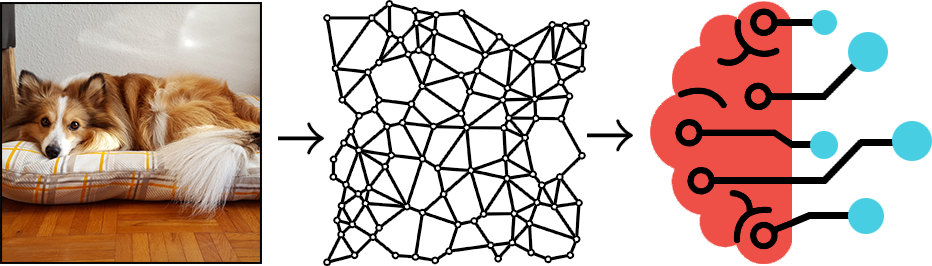
\includegraphics[width=0.9\textwidth]{bilder/problemstellung.png}
\caption[Problemstellung]{Bilder werden in dieser Arbeit für ihre Eingabe in ein neuronales Netz zuvor in eine korrespondierende Graphrepräsentationen konvertiert\protect\footnotemark.}
\label{fig:problemstellung}
\end{figure}
\footnotetext{\url{https://www.shutterstock.com/g/ArtRoseStudio}}

\section{Aufbau der Arbeit}
\label{aufbau_der_arbeit}

Die vorliegende Arbeit gliedert sich, neben den in Kapitel~\ref{grundlagen} vorgestellten Grundlagen, die für das weitere Verständnis der Arbeit von Nöten sind, in vier Bereiche:

Das Kapitel~\ref{graphrepraesentationen_von_bildern} widmet sich der Gewinnung einer Graphrepräsentation aus einem Bild.
Dabei werden insbesondere zwei Verfahren zur Generierung eines Graphen aus einem Bild vorgestellt — die herkömmliche Gitterrepräsentation eines Bildes (Kapitel~\ref{gitter}) sowie die Gewinnung eines Graphen aus einer vorberechneten Superpixelrepräsentation (Kapitel~\ref{superpixel}).

Kapitel~\ref{raeumliches_lernen} und~\ref{spektrales_lernen} erläutern die beiden unterschiedlichen Ansätze des graphbasierten Lernens in neuronalen Netzen — das räumliche und das spektrale Lernen — getrennt voneinander.
Beide Verfahren umfassen den aktuellen Stand der wissenschaftlichen Forschung auf diesem Gebiet.
Zu jedem Ansatz finden sich in den Unterkapiteln~\ref{raeumliche_erweiterung} \bzw{}~\ref{gcn_erweiterung} entwickelte Erweiterungen \bzgl{} der beschriebenen Problemstellung.

Kapitel~\ref{evaluation} evaluiert die vorgestellten sowie entwickelten Ansätze anhand der gegebenen Problemstellung im Vergleich zueinander sowie im Vergleich zu klassischen Lösungen auf diesem Gebiet.
Dazu wird zunächst in Unterkapitel~\ref{versuchsaufbau} der Versuchsaufbau erläutert und dessen Ergebnisse in den Unterkapiteln~\ref{ergebnisse} und~\ref{laufzeitanalyse} präsentiert.
In Kapitel~\ref{ausblick} folgt ein abschließender Ausblick zu möglichen weiterführenden Arbeiten.

